\documentclass{report}
\usepackage[utf8]{inputenc}
\usepackage[francais]{babel}  
\usepackage[T1]{fontenc} 
\usepackage{graphicx}
\usepackage{listings}
\renewcommand{\thesection}{\arabic{section}}
\begin{document}
\title{%
    \begin{minipage}\linewidth
        \centering
        Projet Architecture des Ordinateurs Avancée (Sujet 8)
        \vskip 3pt
        \author{ Marina BLE & Doha ROUIBAA & Pablo BOURDELAS & Guillaume RYCKAERT }
    \end{minipage}
}
\maketitle

\topskip0pt
\vspace*{\fill}
\begin{centering}
    A Etienne le bolideur, et l'effet Vega-Missil.
\end{centering}
\vspace*{\fill}
\newpage


\chapter*{Sujet}

L'objectif de ce projet est d'optimiser la boucle de calcul suivante:
\lstinputlisting[language=c]{../kernel_ref.c}
Le but final de ce projet et de combiner des optimisations dans le code de la boucle et au niveau du compilatuer afin d'avoir la plus grande valeur de speedup possible par rapport a la version ci-dessus, compilée avec gcc -O3.\\

Dans une première partie, nous détaillerons les conditions de test; nous verrons ensuite les optimisations compilateur. Enfin, nous verrons les optimisations au niveau du code.

\chapter*{Partie Meusure}

\section*{Caractéristiques de la machine}

\begin{figure}[ht!]
        \centering
        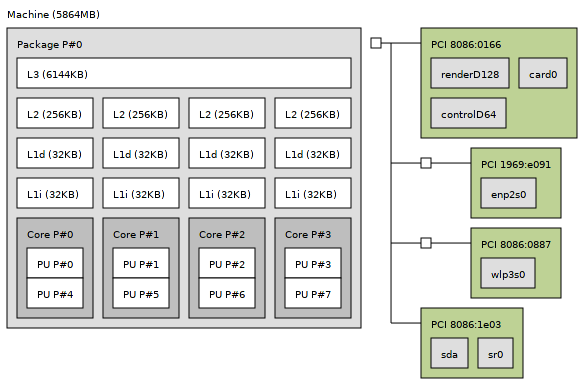
\includegraphics[width=100mm]{MEDIA/Topo.png}
        \caption{Caractéristiques de la machine utilisée}
    \end{figure}

\subsection*{Hardware}

\begin{itemize}
    \item{- I7 3630QM (~Fin 2012) :}
    \item{- 4 cores - 8 threads}
    \item{- Freq : ~2.4Ghz (Idle 1.2Ghz - Turbo mode 3.40 Ghz )}
    \item{- Cache L1: 32Ko}
    \item{- Cache L2: 256Ko}
    \item{- Cache L3: 6 144Ko}
    \item{- 6 Go de RAM:  La capacité en RAM est répartie sur 2 unités: une de 4 et une de 2 Go, celà nous empêche d'utiliser du dual channel. De plus les unités sont plutôt bas de gamme.}
\end{itemize}

\subsection*{Système}

\begin{itemize}
    \item{- gcc 6.3.1}
    \item{- Arch x86\_64 ( noyaux Linux 4.10.6-1 Arch )}
\end{itemize}

\section*{Détermination de la taille des données}

Notre boucle a besoin de 3 tableaux de taille n et d'un tableau de taille n$\times$n.\\
Chaque case du tableau prend 4 octets (int32\_t/float)\\
Le coût total en mémoire est donc de $4n^2+12n$ octets.\\

On résoud les équations du second degré selon les tailles du cache:\\

\subsection*{Cache L1}
Pour être sur que les donnés tiennent en L1, on fait le calcul avec $5\%$ de marge.
Le cache L1 fait 32Ko, notre équation est donc $4n^2+12n=(32 000*0.95)=30 400$
La solution trouvée est $\approx 85.6509$, il faut donc prendre des tableaux de 85 cases. Coût total: 29.920 Ko.\\

\subsection*{Cache L2}
Pour le L2, on prenda $10\%$ de marge sur la taille du L2.
Le cache L2 fait 256Ko, notre équation est donc $4n^2+12n=(256 000*0.9)=230 400$\\
La solution trouvée est $\approx 238.505$, il faut donc prendre des tableaux de 238 cases. Coût total: 229.432 Ko.\\

\subsection*{Cache L3}
Pour le L3, on prendra $50\%$ de marge sur la taille du L3.
Le cache L3 fait 6144Ko, notre équation est donc $4n^2+12n=(6 144 000*0.5)= 3 077 000$\\
La solution trouvée est $\approx 875.57$, il faut donc prendre des tableaux de 875 cases. Coût total: 3 073.000 Ko.\\

\subsection*{En RAM}
En RAM, nous prendons 3x la taille du cache L3,pour être sur que nos données soient mises en RAM.
Notre équation est donc $4n^2+12n=(6 144 000*3)=18 432 000$\\
La solution trouvée est $\approx 2145.13$, il faut donc prendre des tableaux de 2145 cases. Coût total: 18 429.840 Ko.\\

\begin{tabular}{ l c | c c }
    Type de Mémoire & Taille Mémoire & Taille Tableau & Coût Total\\\hline
    L1 & 32Ko & 85 & 29.920 Ko\\ 
    L2 & 256Ko & 238 & 229.432 Ko \\
    L3 & 6 144Ko & 875 & 3 073.000 Ko \\
    RAM & 5 864Mo & 2145 & 18 429 840 Ko \\
\end{tabular}

\section*{Détermination du nombre de cycles de Warmup}

Pour déterminer le nombre de cycles de warmup nécessaires: On lance plusieurs fois la boucle de warmup, et l'on trace le graphe du temps d'éxécution en fonction du nombre de répétitons successives.

On détermine ensuite le nombre de répétitons nécéssaires par méthode graphique.

Pour vérifier nos résultats, les tests ont également été effectués pour 200 000 tours.
On sépare les cas pour les différentes tailles de données:

\newpage
\subsection*{Warmup en Cache L1}
    \begin{figure}[ht!]
        \centering
        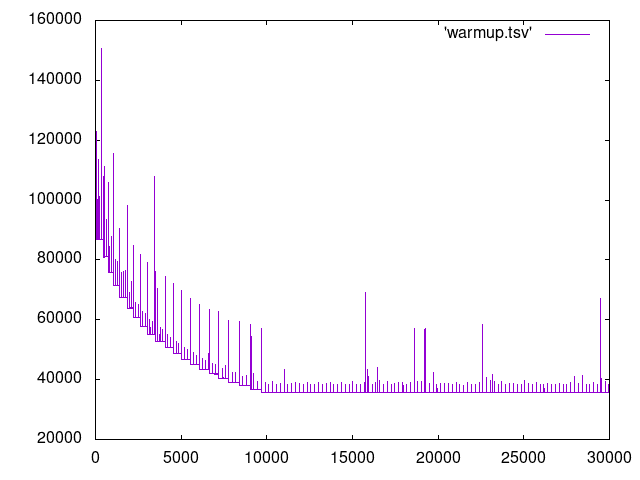
\includegraphics[width=120mm]{MEDIA/warmupL1_Cstate.png}
        \caption{Warmup en cache L1 avec tout Cstate autorisé}
    \end{figure}

On remarque que le warmup est relativement long, en désactivant les Cstates,celui-ci devient plus court.\\

En effet, les Cstates permettent d'économier l'énergie consommée par le processeur en endormant certains composants, qui peuvent être long a réveiller.\\

Sans Cstates, le proceseur n'a que 3 états: Idle, Normal et Turbo, et passe donc très rapidement en mode turbo.\\
\newpage
    \begin{figure}[ht!]
        \centering
        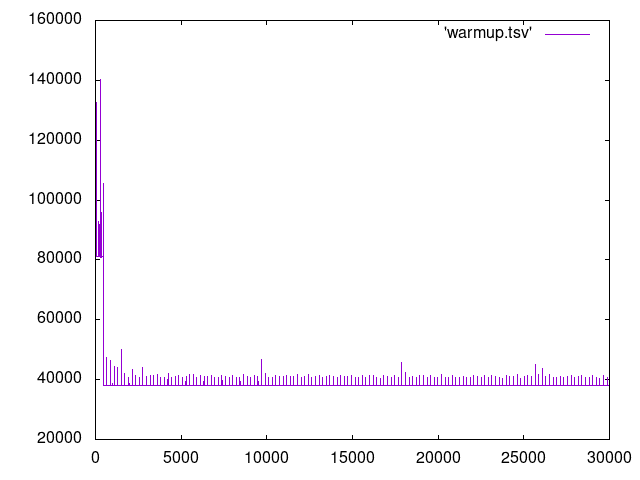
\includegraphics[width=120mm]{MEDIA/warmupL1_NOCstate.png}
        \caption{Warmup en cache L1 avec Cstate max=0}
    \end{figure}

Il nous faut donc 2000 cycles de warmup pour une taille de données rentrant en cache L1.\\

Pour la suite, nous continuons à faire nos calculs avec Cstate max=0
\newpage

\subsection*{Warmup en Cache L2}
    \begin{figure}[ht!]
        \centering
        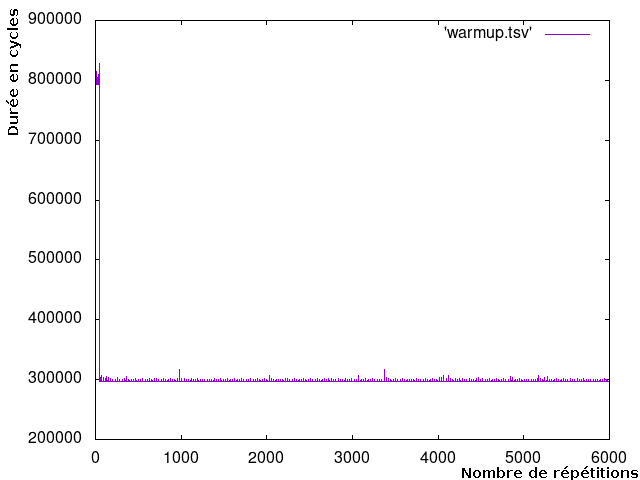
\includegraphics[width=120mm]{MEDIA/warmupL2_NOCstate.png}
        \caption{Warmup en cache L2}
    \end{figure}

On constate que les temps de calculs deviennent rapidement stables.

\newpage
    \begin{figure}[ht!]
        \centering
        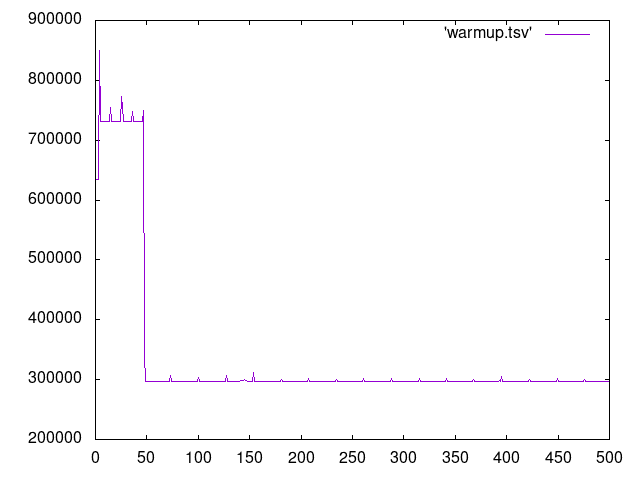
\includegraphics[width=120mm]{MEDIA/closeup.png}
        \caption{Warmup en cache L2}
    \end{figure}

    On décide de prendre 500 cycles de warmup pour avoir une marge.

\newpage
\subsection*{Warmup en Cache L3}
    \begin{figure}[ht!]
        \centering
        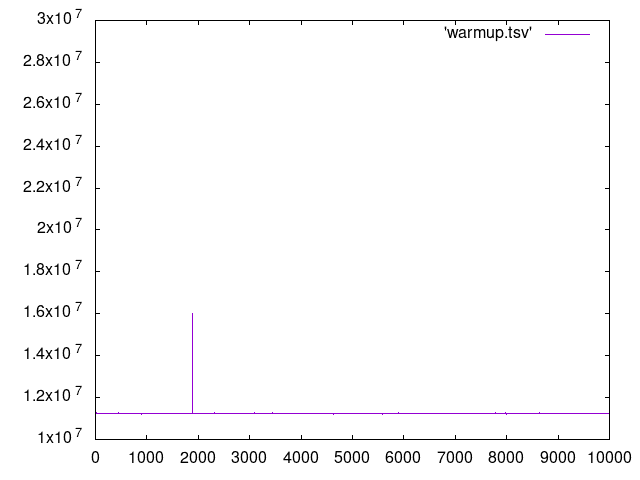
\includegraphics[width=120mm]{MEDIA/warmupL3_NOCstate.png}
        \caption{Warmup en cache L3}
    \end{figure}

Au niveau du L3, Nous avons commencé par tester pour 10 000 éxécutions. 

\newpage 
    \begin{figure}[ht!]
        \centering
        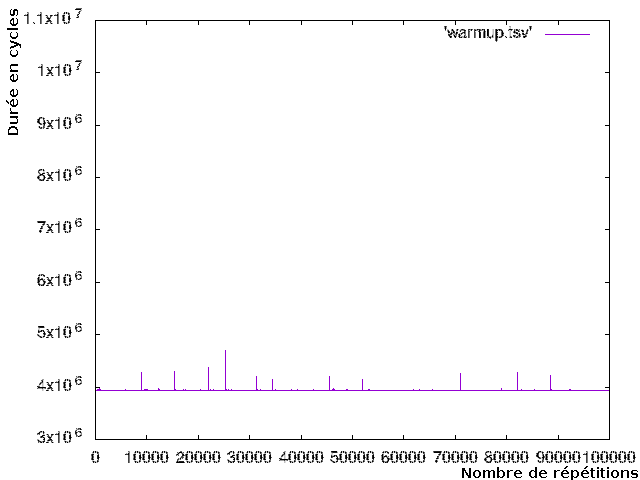
\includegraphics[width=120mm]{MEDIA/warmupL3_100000.png}
        \caption{Warmup en cache L3 }
    \end{figure}

On remarque, que pour 100 000 éxécutions, le programme finit plus vite à chaque fois!
On décide donc de tester pour 200 000 éxécutions.

\newpage
    \begin{figure}[ht!]
        \centering
        
\includegraphics[width=120mm]{MEDIA/warmupL3_200000.png}
        \caption{Warmup en cache L3 }
    \end{figure}

    On constate que pour les ~30K premières éxécutions, le temps de calcul est le même que pour chacune des 10 000. Il descend ensuite à la valeur obtenue pour chaque boucle des 100 000 tours de warmup.Nous avons donc decidé de prendre 50K tours de warmup, ce qui nous donne un résultat similaire au 100K d'après nos tests.
   \newpage

\subsection*{Warmup en RAM}
   \begin{figure}[ht!]
        \centering
        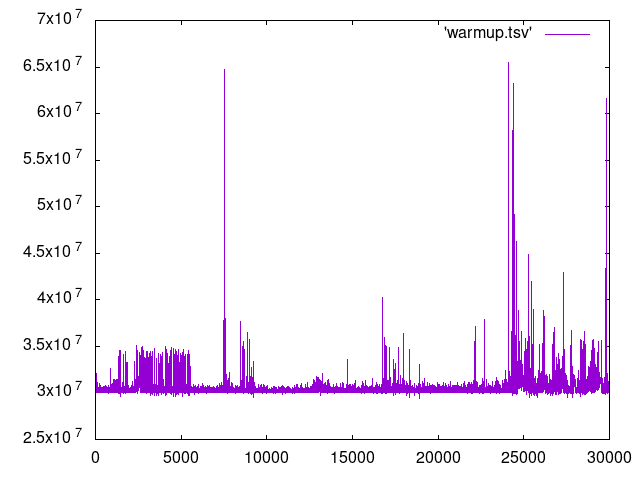
\includegraphics[width=120mm]{MEDIA/warmupRAM.png}
        \caption{Warmup en RAM }
    \end{figure}
En RAM, le temps d'éxécution est très inconsistant, en regardant le graphique de plus près, on constate qu'il n'y a quasiment pas besoin de warmup. C'est pour cela que l'on décide de prendre que 200 tours.

\section*{Nombre de répétitions}



\section*{Nombre de méta-répétitions}


\chapter*{Flags d'optimisation}

On a éssayé différents flags de compilation suivant le processeur.

\section*{Pour gcc}
\begin{itemize}
    \item{-Og: n'active que les optimisations triviales. Nous avons choisi de tester ce flag uniqument pour voir si les optimisations avait un quelconque effet}
    \item{-O3: référence, nous avons pu voir avec maqao que la puissance processeur reste mal exploité notament à cause du manque de vectorisation, option pourtant activé.}
    \item{-Ofast: Optimisation agressive, violation de certains standards IEEE. Ce flag devrait permettre d'accélérer la division présente }
    \item{-funsafe-math-optimizations : compris dans -Ofast, IEEE non-strict. Ce flag est compris dans Ofast nous l'avons tester à part pour voir si la totalité de Ofast était utile } 
    \item{-ffast-math: Flottants non associatifs + IEEE non stricts.}
    \item{-frename-registers: technique de renommage de registres, pour éliminer certaines dépendances inter-instructions}
    \item{-fsection-anchors: Optimisation agressive sur les accés mémoire pour diminuer le calcul d'adresse-non disponble sur l'architecture cible}
\end{itemize}

\section*{Pour icc}
\begin{itemize}
    \item{-O3 niveau d'optimisation équivalent à celui de gcc}
    \item{-fast : optimistation ultra agressive, qui donne un code très rapide, mais il nous était impossible de l'anaylser avec maqao. Quelques doutes subsistaient sur sa consistance, avant l'examen du listing assembleur}
    \item {-Ofast: similaire à gcc}
\end{itemize}   

\section*{Comparaisons}

\subsection*{Temps en L1}
\begin{figure}[ht!]
\centering
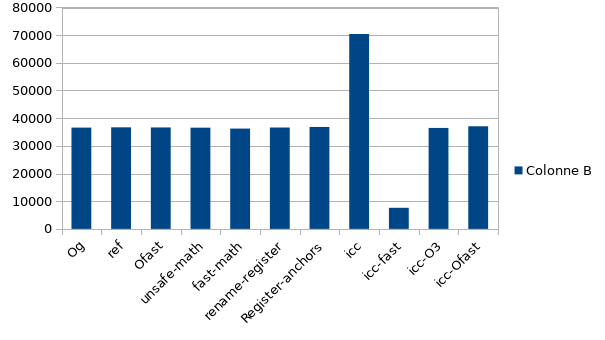
\includegraphics[width=120mm]{MEDIA/time_L1.png}
\caption{Temps selon les flags utilisés en L1}
\end{figure}
On remarque que icc avec le flag fast, génère un code bien plus rapide que gcc.
Cela vient du fait que bien qu'elle soit activée, gcc ne vectorise pas le code.\\
Comme dit plus haut nous n'avons pas pu faire l'analyse du binaire généré avec icc -fast avec maqao. En effet les résultats de maqao fournis n'étaitent pas cohérents
 ( nombre de boucles différent entre 2 expériences sur un binaire identitique, instructions non reconnues, etc ). Nous avons donc décidé d'eximiner le listing assembleur produit pour le kernel,\\
 avec icc sans flag ( autre que -S pour obtenir le listing ) et icc -fast. La première différence est la zone des ".byte" ne connaissant pas assez bien l'assembleur nous ne savons pas à quoi cette zone servait.
La deuxième est qu'une bonne partie des instructions scalaires ont été remplacées par des instructions vectorielles AVX
( movss -> vmovss, divss -> vdivss ). On peut aussi observer que la double boucle a été deroulée, ce qui est déjà le cas sans flag. Nous avons aussi regardé le listing généré pour gcc en O3 ce qui nous a bien confirmé qu'aucune vectorisation n'a été appliquée.
\newpage
\subsection*{Temps en L2}
\begin{figure}[ht!]
    \centering
    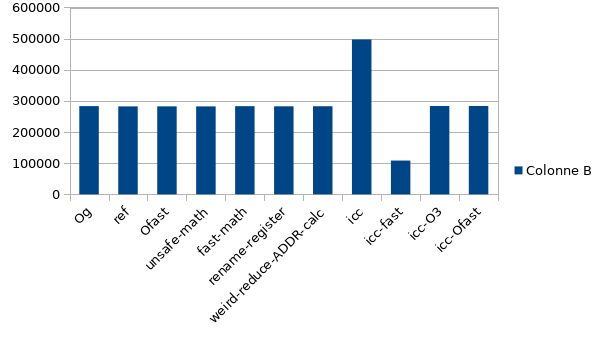
\includegraphics[width=120mm]{MEDIA/Resultat_TEST_L2.png}
    \caption{Temps selon les flags utilisés en L2}
\end{figure}
\subsection*{Temps en L3}
\begin{figure}[ht!]
    \centering
    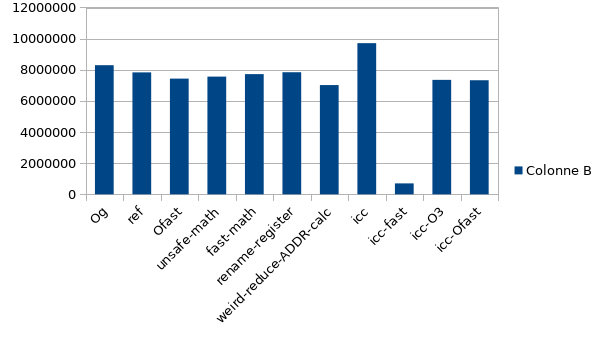
\includegraphics[width=120mm]{MEDIA/Resultat_TEST_L3.png}
    \caption{Temps selon les flags utilisés en L3}
\end{figure}



\chapter*{L'Optimisation du Code}
\section*{La division}

L'opération la plus lognue dans notre kernel est la division. A chaque exécution du kernel, celle-ci est éxécutée $n^2$ fois.

On inverse les boucles, ainsi on ne fait plus que $n$ divisions ; mais on doit faire en plus $n^2$ multiplications par appel du kernel.
\\Sur les processeurs Ivy Bridge, la multiplication est environ 3$\times$ plus rapide que la divsion. En considérant qu'une multiplication est faite en 1 cycle, on peut donc comparer.
Sans les boucles inversées,le traitement fait $n^2$ divsions, pour une durée de $3n^2$.
Avec les boucles inversées,le traitement fait $n$ divisions et $n^2$ multiplications, soit une durée de $3n+n^2$.
On compare $3n^2$ et $3n+n^2$:\\
\begin{figure}[ht!]
    \centering
    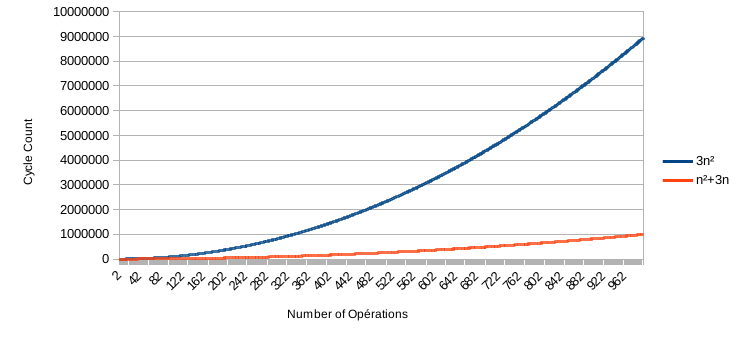
\includegraphics[width=100mm]{MEDIA/div_vs_mult_graph.png}
    \caption{Comparaison des temps de calcul des deux méthodes}
\end{figure}
Inverser les boucles est donc beaucoup plus rentable.
Speedup offert par cette optimisation:$\approx 3.11$.

\section*{Vectorisation}

La vectorisation est la possiblité de faire plus rapidement le même type d'opération a la suite, grâce a l'utilisation d'instructions et de registres particuliers.Le code peut être écrit de manière vectorisée, via l'utiliation d'intrinsics, ou bien cette optimisation peut-être faite par le compilateur.

Nous avons tenté dans un premier temps de vectoriser le code a la main, ce qui nous permettait d'atteindre $100\%$ de vectorisation.  Cepedant les résultats devenaient très peu consitants, c'est pourquoi nous avons décidé laisser le compilateur vectorsier le code a notre place.

Malheusement cela etait impossible a cause de l'accès indirect; Nous avons donc cherché un moyen de le retier.
\subsection*{L'accès indirect}
Cette méthode est faisable grâce a notre inversion de boucles.

Nous proposons d'ajouter une boucle au début du noyeau qui calculera les accés indrects avant que ceux-ci soient utilisés dans la bocule de calcul.
Ces données doivent être stockées entre le temps, la première idée serait d'ajouter un tableau supplémentaire a cet effet, mais il faudrait alors recalculer toutes les tailles de tableau pour le L1, L2, L3 et RAM (n valeurs supplémentaires a stocker).\\

Pour ne pas consommer plus de mémoire, nous avons donc décidé de stocker ces valeurs sur la dernière ligne du tableau résultat.
Lors du calcul de la dernière ligne, l'indice indirect est donc lu pour la dernière fois juste avant d'être remplacé par le résultat. 

\subsection*{Vectorisation compilateur}

Avant de supprimer l'accès indirect via la 1ère boucle, il était impossible pour les compilateurs de vectoriser le code.

Maintenant nous avons un code vectorisé a:
    \begin{itemize}
    \item{$66\%$ avec gcc}
    \item{$75\%$ avec icc}
    \end{itemize}

    Le code est vectorisé avec des instructions AVX, qui utilisent des registres de 256 bits. On peut donc stocker 8 floats/int32\_t par registre AVX.
    Il n'est pas vraiment possible de donner le speedup individuel de cette optimisation, car elle dépend de l'inversion des boucles.
Speedup avec ces deux optimisations :$\approx 7.11$
\section*{Tiling}
Nous avons également envisagé de faire du tiling. Le tiling est une méthode consistant a découper le traitement de la matrice en un ensemble de sous-traitements sur des sous-ensembles de cette matrice..Ces matrices étant plus petites, elle peuvent être chargées dans des niveaux de cahche plus rapides, et donc accélérer le traitement.
Malheursement, nous nous sommes rapidement rendus compte que cette méthode n'était pas adaptée a notre traitement.
En effet le tiling a un intérêt seulment quand une même partie de matrice est réutilisée plusieurs fois, ce qui n'est pas notre cas.
De plus, cela nuirait a notre optimisation sur la division, si par exemple on découpe notre matrice en 100 blocs de même taille, il nous faudra faire $10\times n $ divisions.

Nous n'avons donc pas appliqué cette methode.

\section*{Optimisations Compilateur}

Nous avons également utilisé un flag de compilation supplémentaire, afin d'aller toujours plus vite.
Ce flag s'écrit --march=native pour gcc et -xHost pour icc. Il indique au compilateur que le code est destiné exculsivement au processeur utilisé pour la compilation, et permet donc une optimisation plus poussée.\\
\begin{itemize}
    \item{Speedup pour gcc (Avec les autres opti):$\approx 8.97$}
    \item{Speedup pour icc (Avec les autres opti):$\approx 11.30$}\\
\end{itemize}

\section*{Cohérence des résultats}

A chaque étape de l'optimisation, nous avons contrôlé la cohérence des résultats. Pour cela, nous avons utilisé vim, et gardé une valeur constante depuis le début du projet pour générer nos valeurs aléatoires. La plus grosse perte de précision que nous ayons trouvé est de l'ordre de $10^{-6}$


\section*{Répartition des tâches}
Chaque membre du groupe a effectué des calculs sur une taille de données:
\begin{tabular}{ l | c }
    Membre & Taille de données \\\hline
    Marina & RAM \\
    Doha & L3\\
    Pablo & L1\\
    Guillaume & L2\\
\end{tabular}
\section*{Conclusion}
Ce projet nous a permis d'approfondir nos connaissances en matière d'optimisation de code, que ce soit par la découverte d'icc (gcc étant le seul compilateur c que nous ayons utilisé jusqu'a présent), mais aussi par celle d'outils permettant de meusurer la performance du code, comme maqao.

Nous avons également mesuré la rigeur nécessaire pour créer des conditions de test stables, qui nous permettent d'obtenir des résultats valables, d'où la nécéssité d'une bonne répartition des tâches.


\end{document}
